\documentclass[a4paper, 12pt]{article}%тип документа

%отступы
\usepackage[left=1.5cm,right=1cm,top=2cm,bottom=3cm,bindingoffset=0cm]{geometry}
\setlength{\parindent}{5ex}

%Русский язык
\usepackage[T2A]{fontenc} %кодировка
\usepackage[utf8]{inputenc} %кодировка исходного кода
\usepackage[english,russian]{babel} %локализация и переносы

%Вставка картинок
\usepackage{graphicx}
\graphicspath{{pictures/}}
\DeclareGraphicsExtensions{.pdf,.png,.jpg,.jfif}
\usepackage{wrapfig}

%Графики
\usepackage{pgfplots}
\pgfplotsset{compat=1.9}

%Математика
\usepackage{amsmath, amsfonts, amssymb, amsthm, mathtools}

%Таблицы
\usepackage{longtable} 
\usepackage{float}

%Римские цифры
\newcommand{\RomanNumeralCaps}[1]{\uppercase\expandafter{\romannumeral#1}}

\usepackage{multirow}


\begin{document}
	\begin{titlepage}
		\begin{center}
			\textsc{Федеральное государственное автономное образовательное учреждение высшего образования«Московский физико-технический институт (национальный исследовательский университет)»\\[5mm]
			}
			
			\vfill
			
			\textbf{Отчёт по лабораторной работе 5.1.2\\[3mm]
				Исследование эффекта Комптона
				\\[50mm]
			}
			
		\end{center}
		
		\hfill
		\begin{minipage}{.5\textwidth}
			Выполнил студент:\\[2mm]
			Сериков Василий Романович\\[2mm]
			Сериков Алексей Романович\\[2mm]
			группа: Б03-102\\[5mm]
			
		\end{minipage}
		\vfill
		\begin{center}
			Москва, 2023 г.
		\end{center}
		
	\end{titlepage}
	
	\newpage
	\setcounter{page}{2}
	\textbf{Аннотация}\\
	
	\textbf{Цель работы: }\\
	 С помощью сцинтилляционного спектрометра исследуется энергетический спектр $\gamma$ - квантов, рассеянных на графите. Определяется энергия рассеянных $\gamma$ -квантов в зависимости от угла рассеяния, а также энергия покоя частиц, на которых происходит комптоновское рассеяние.\\
	
	\textbf{Теория: }\\
	Рассеяние $\gamma$ -лучей в веществе относится к числу явлений, в которых особенно ясно проявляется двойственная природа излучения. Волновая теория, хорошо объясняющая рассеяние длинноволнового излучения, испытывает трудности при описании рассеяния рентгеновских и $\gamma$ -лучей. Эта теория, в частности, не может объяснить, почему в составе рассеянного излучения, измеренного Комптоном, кроме исходной волны с частотой $\omega_{0}$ появляется дополнительная длинноволновая компонента, отсутствующая в спектре первичного излучения.
	
	Появление этой компоненты легко объяснимо, если считать, что $\gamma$-излучение представляет собой поток квантов (фотонов), имеющих энергию $\hbar \omega$ и импульс $p=\hbar \omega / c .$ Эффект Комптона - увеличение длины волны рассеянного излучения по сравнению с падающим - интерпретируется как результат упругого соударения двух частиц: $\gamma$ -кванта (фотона) и свободного электрона.
	
	Рассмотрим элементарную теорию эффекта Комптона. Пусть электрон до соударения покоился (его энергия равна энергии покоя $m c^{2}$ ), a $\gamma$ -квант имел начальную энергию $\hbar \omega_{0}$ и импульс $\hbar \omega_{0} / c .$ После соударения электрон приобретает энергию $\gamma m c^{2}$ и импульс $\gamma m v,$ где $\gamma=$ $=\left(1-\beta^{2}\right)^{-1 / 2}, \beta=v / c,$ a $\gamma$ -квант рассеивается на некоторый угол $\theta$ по отношению к первоначальному направлению движения. Энергия и импульс $\gamma$ -кванта становятся соответственно равным и $\hbar \omega_{1}$ и $\hbar \omega_{1} / c($ рис. 1$)$. Запишем для рассматриваемого процесса законы сохранения энергии и импульса:
	$$
	\begin{array}{c}
		m c^{2}+\hbar \omega_{0}=\gamma m c^{2}+\hbar \omega_{1} \\
		\frac{\hbar \omega_{0}}{c}=\gamma m v \cos \varphi+\frac{\hbar \omega_{1}}{c} \cos \theta \\
		\gamma m v \sin \varphi=\frac{\hbar \omega_{1}}{c} \sin \theta
	\end{array}
	$$
	Решая совместно эти уравнения и переходя от частот $\omega_{0}$ и $\omega_{1}$ к длинам волн $\lambda_{0}$ и $\lambda_{1},$ нетрудно получить, что изменение длины волны рассеянного излучения равно
	\begin{equation}
		\Delta \lambda=\lambda_{1}-\lambda_{0}=\frac{h}{m c}(1-\cos \theta)=\Lambda_{\mathrm{K}}(1-\cos \theta)
	\end{equation}
	где $\lambda_{0}$ и $\lambda_{1}$ - длины волн $\gamma$ -кванта до и после рассеяния, а величина
	$$
	\Lambda_{\mathrm{K}}=\frac{h}{m c}=2,42 \cdot 10^{-10} \text{см}
	$$
	
	Основной целью данной работы является проверка соотношения
	(1). Применительно к условиям нашего опыта формулу
	(1) следует преобразовать от длин волн к энергии $\gamma$ -квантов. Как нетрудно показать, соответствующее выражение имеет вид
	\begin{equation}
		\frac{1}{\varepsilon(\theta)}-\frac{1}{\varepsilon_{0}}=1-\cos \theta
	\end{equation}
	Здесь $\varepsilon_{0}=E_{0} /\left(m c^{2}\right)-$ выраженная в единицах $m c^{2}$ энергия $\gamma$ -квантов, падающих на рассеиватель, $\varepsilon(\theta)$ - выраженная в тех же единицах энергия квантов, испытавших комптоновское рассеяние на угол $\theta, m-$ масса электрона.\\
	
	
	\textbf{Экспериментальная установка: }\\
	Блок-схема установки изображена на рис. $3 .$ Источником излучения 1 служит $^{137} \mathrm{Cs},$ испускаюший $\gamma$ -лучи с энергией 662 кэВ. Он помещен в толстостенный свинцовый контейнер с коллиматором. Сформированный коллиматором узкий пучок $\gamma$ -квантов попадает на графитовую мишень 2 (цилиндр диаметром 40 мм и высотой 100 мм).
	
	\begin{figure}[h]
		\begin{center}
			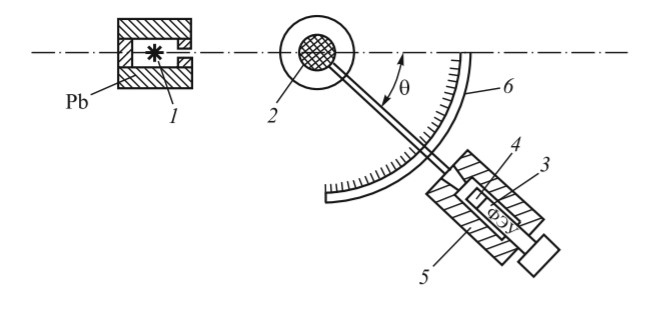
\includegraphics[width = \textwidth]{16.jpg}
			\caption{Экспериментальная установка}
		\end{center}
	\end{figure}
	
	Кванты, испытавшие комптоновское рассеяние в мишени, регистрируются сцинтилляционным счетчиком, принцип работы которого рассмотрен в работе 5.3. Счетчик состоит из фотоэлектронного умножителя 3 (далее ФЭУ) и сцинтиллятора $4^{*}$ ). Сцинтиллятором служит кристалл NaI(Tl) цилиндрической формы диаметром 40 мм и высотой 40 мм, его выходное окно находится в оптическом контакте с фотокатодом ФЭУ. Сигналы, возникающие на аноде ФЭУ, подаются на ЭВМ для амплитудного анализа. Кристалл и ФЭУ расположены в светонепроницаемом блоке, укрепленном на горизонтальной штанге. Штанга вместе с этим блоком может вращаться относительно мишени, угол поворота отсчитывается по лимбу $6 .$
	
	Пусть $\varepsilon(\theta) = AN(\theta)$, $A$ -- коэффициент пропорциональность, $N(\theta)$ -- номер соответствующего канала. Тогда (2) перепишется как
	\begin{equation}
		\dfrac{1}{N(\theta)} - \dfrac{1}{N(0)} = A(1-\cos \theta).\
	\end{equation}
	Отсюда можно определить энергию покоя электрона как 
	\begin{equation}
		mc^2 = E_\gamma \dfrac{N(90)}{N(0) - N(90)},
	\end{equation}
	где $E_\gamma = E_0$ -- энергия испускаемых источником $\gamma$-квантов.
	
	
	
	
	
	
	
	
	
	
	
	
	
	
	
	
	
	\end{document}